\documentclass[notitlepage, 11pt]{report}


% Packages
% --------
%	 Necessary
\usepackage{geometry} 						% geometry - page dimensions
\usepackage[parfill]{parskip}				% parskip - to use blank line to sep paragraphs
\usepackage{titling}						% title formatting
\usepackage{enumitem}

\usepackage{amsmath}						% AMS - math, fonts, symbols, theorem
\usepackage{amsfonts}
\usepackage{amssymb}
\usepackage{amsthm}
\usepackage{mathtools}						% mathtools - \coloneqq

\usepackage{listings}						% listings - prints source code

\usepackage{hyperref}						% hyperref - urls and things

\usepackage{tikz}							% tikz - graphs

% 	Additional
\usepackage{graphicx}						% graphicx - importing graphics from file
\usepackage{subcaption}
\captionsetup[subfigure]{labelformat=empty}
\usepackage[T1]{fontenc}
\usepackage[utf8]{inputenc}
\usepackage{helvet}
\renewcommand{\familydefault}{\sfdefault}	% change to helvetica

\usepackage{forest}							% forest - easy trees
\usepackage{tikzsymbols}					% tikzsymbols - just adds some symbols
% tikzlibrary summary: 
% tex.stackexchange.com/questions/42611/list-of-available-tikz-libraries-with-a-short-introduction/491626
\usetikzlibrary{arrows.meta}				% arrows.meta - customizable arrow tips
\usetikzlibrary{er}							% entity-relationship diagrams
\usetikzlibrary{positioning} 				% relative positioning
\usetikzlibrary{shadows}
\usetikzlibrary{shapes}

\usepackage{xcolor}							% xcolor - adds additional colors

\usepackage{marginnote}						% marginnote - see name

\usepackage{multirow}						% multirow - sort of a tabular environment of text
\usepackage{bigdelim}						% bigdelim - used with multirow once to make brackets on tables
\usepackage{array}							% array - extends arrary and tabular environment
\usepackage{makecell}						% makecell - adjust cell cizes within tabular environment

\usepackage[bottom]{footmisc}				% comment out to make footnotes not appear at bottom of page

% Customizations

\pretitle{\begin{center}\Large\bfseries}		% titling format
\posttitle{\par\end{center}\vskip 0cm}
\preauthor{\begin{center}\large}
\postauthor{\end{center}}
\predate{\par\normalsize\centering}
\postdate{\par}

\newtheoremstyle{customnumber} % name
	{}% space above
	{}% space below
	{\normalfont}% body font
	{}% indent 
	{\bfseries}% head font
	{:}% punctuation between head/body
	{ }% space after head: " " = normal whitespace
	{\thmname{#1}\thmnote{ #3}}% head format

\newtheoremstyle{named}
	{}
	{}
	{\normalfont}
	{}
	{\bfseries}
	{.}
	{ }
	{\thmnote{#3}}

\theoremstyle{customnumber}
\newtheorem*{exercise}{Exercise}

\theoremstyle{definition}
\newtheorem{defi}{Definition}

\newtheorem{ex}{Example}[section]

\theoremstyle{named}
\newtheorem*{namedtheorem}{}

\newenvironment{absolutelynopagebreak}
	{\par\nobreak\vfil\penalty0\vfilneg\vtop\bgroup}
	{\par\xdef\tpd{\the\prevdepth}\egroup\prevdepth=\tpd}
	
\newcommand{\indep}{\raisebox{0.05em}{\rotatebox[origin=c]{90}{$\models$}}}

\newcommand{\stcomp}[1]{{#1}^\complement}


\lstset{tabsize=3, numbers=left, basicstyle=\ttfamily, escapeinside=~~, xleftmargin=-1cm}
\let\origthelstnumber\thelstnumber
\makeatletter
\newcommand*\Suppressnumber{%
	\lst@AddToHook{OnNewLine}{%
		\let\thelstnumber\relax%
		\advance\c@lstnumber-\@ne\relax%
	}%
}
\newcommand*\Reactivatenumber{%
	\lst@AddToHook{OnNewLine}{%
		\let\thelstnumber\origthelstnumber%
		\advance\c@lstnumber\@ne\relax%
	}%
}
\makeatother

\geometry{left=1in, right=1in, top=1in, bottom=1in}

\title{COMP3700 Assignment 3}
\author{Tripp Isbell\\
	\texttt{cai0004@auburn.edu}}
\date{}

\begin{document}
\maketitle
For the first version of the store mangement system, we want to start with the following user stories:
\begin{itemize}
	\item As a user, I want to add a new product into the system.
	\item As a user, I want to add a new customer into the system.
	\item As a user, I want to record a purchase from a customer into the system.
\end{itemize}
\begin{enumerate}[itemindent=-1.5em]
	\item Write a common use case for each user story. Sketch the screens the system should display in each use case.
	
	\textbf{Use Case:} add a product into the system\\
	\textbf{Actors:} employees\\
	\textbf{Goals:} update database to include new product\\
	\textbf{Related use cases:} adding a customer to the database or recording a transaction (below)
	\textbf{Preconditions:} interface is functional and connected to underlying database\\
	\textbf{Postconditions:} The product database is updated with the item\\
	\textbf{Steps:}
		\begin{itemize}
		\item the user clicks a button to display the product database
		\item the system displays the database
		\item the user clicks a plus button 
		\item the system displays a screen with text fields for the product info
		\item the user enters the information and clicks an add button
		\item the system updates the database and displays a confirmation message
		\item the user clicks confirm 
		\item the system returns to the main menu
		\end{itemize}
	\textbf{Use case:} add a customer into the system\\
	\textbf{Actors:} employees\\
	\textbf{Goals:} update database to include new customer\\
	\textbf{Related use cases:} adding a product (above) or transaction (below)
	\textbf{Preconditions, steps, postconditions:} Same as above just replace "product" with "customer"
		\textbf{Steps:}
		\begin{itemize}
		\item the user clicks a button to display the customer database
		\item the system displays the database
		\item the user clicks a plus button 
		\item the system displays a screen with text fields for the customer info
		\item the user enters the information and clicks an add button
		\item the system updates the database and displays a confirmation message
		\item the user clicks confirm 
		\item the system returns to the main menu
		\end{itemize}
	\textbf{Use case:} record a transaction\\
	\textbf{Actors:} employees\\
	\textbf{Goals:} update transaction records with new transaction (customer, product, price paid)\\
	\textbf{Related use case:} similar to product and customer cases\\
	\textbf{Preconditions:} interface is set up and connected to transaction database, ideally the process is also set up to be somewhat automated\\
	\textbf{Postconditions:} the database is updated with the transaction (ideally the system automatically breaks the purchase of multiple products into atomic purchases of each individual product)\\
\newpage
	\textbf{Steps:} 
		\begin{itemize}
		\item the user clicks add purchase
		\item the system prompts employee to scan barcode
		\item the user scans the barcode 
		\item the system identifies the product
		\item the system displays a prompt for quantity of purchase
		\item the user enters a value into the prompt
		\item the system displays the customer database and a text field for name
		\item the user starts typing the name
		\item the system trims the database as the name is typed
		\item the user selects the customer when they see them
		\item the system displays a customer confirmation prompt
		\item the user clicks confirm
		\item the system displays transaction information (item, customer, price, tax) along with a confirm or cancel button
		\item the user reviews the summary info of the transaction to verify, and then confirms
		\item the system displays a success screen
		\item the user clicks confirm
		\item the system returns to the main menu
		\end{itemize}
	\begin{center} 
	Generic screens (applicable to all three cases):
	
	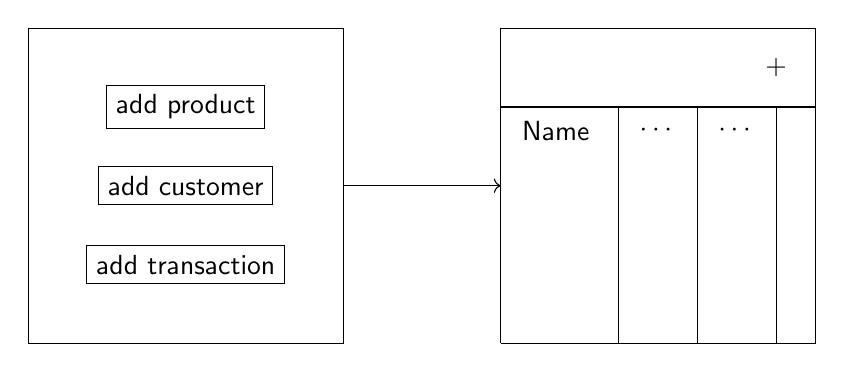
\begin{tikzpicture}
	\draw (0,0) -- (4,0) -- (4,4) -- (0,4) -- (0,0);
	\node[rectangle,draw] (AddProduct) at (2,3) {add product};
	\node[rectangle,draw] (AddCustomer) at (2,2) {add customer};
	\node[rectangle,draw] (AddPurchase) at (2,1) {add transaction};
	\draw[->] (4,2) -- (6,2);
	\draw (6,0) -- (10,0) -- (10,4) -- (6,4) -- (6,0);
	\node (plus) at (9.5,3.5) {+};
	\draw (6,0) -- (10,0) -- (10,3) -- (6,3) -- (6,0);
	\node[rectangle] (Name) at (6.7,2.7) {Name};
	\node[rectangle] (Attributes) at (8, 2.7) {$\cdots$};
	\node[rectangle] (Attributes2) at (9, 2.7) {$\cdots$};
	\draw (7.5,0) -- (7.5,3);
	\draw (8.5,0) -- (8.5,3);
	\draw (9.5,0) -- (9.5,3);
	\end{tikzpicture}
	\end{center}
	\item Draw the entity-relationship diagram for this system. We assume the minimal requirement with two entities: products and customers, and one relationship "a customer purchases a product".
	\begin{center}
	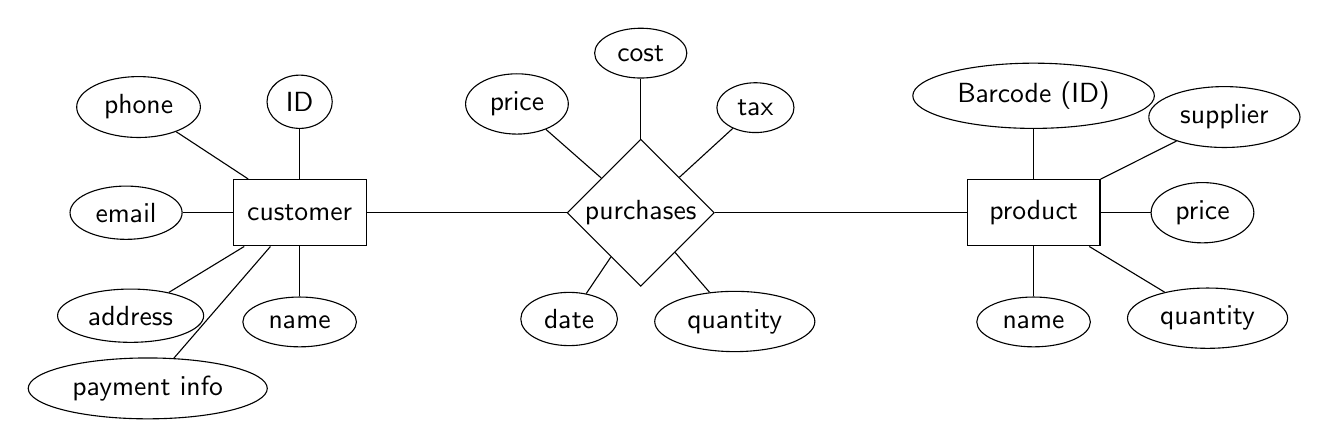
\begin{tikzpicture}
	\node[entity] (customer) {customer};
	\node[entity] (product) [right=3in of customer] {product};
	\node[relationship] (purchases) [right=1in of customer] {purchases}				edge (customer) edge (product);
%	\foreach \i in {-1, 1}{%
%	\draw[-] (customer.east) -- ([yshift=\i * 0.5 em]purchases.west); 
%	\draw[-] (product.west) -- ([yshift=\i * 0.5 em]purchases.east);
%	}
	\node[attribute] (customerID) [above=0.25in of customer] {ID}
	edge (customer);
	\node[attribute] (customerName) [below=0.25in of customer] {name}
	edge (customer);
	\node[attribute] (customerEmail) [left=0.25in of customer] {email}
	edge (customer);
	\node[attribute] (customerAddress) [below left=0.25in and 0.25in of customer] {address}
	edge (customer);
	\node[attribute] (customerPhone) [above left=0.25in and 0.25in of customer] {phone}
	edge (customer);
	\node[attribute] (customerPayInfo) [below left=0.6in and 0in of customer] {payment info}
	edge (customer);
	
	\node[attribute] (purchaseDate) [below left=0.25in and 0in of purchases] {date}
	edge (purchases);
	\node[attribute] (purchaseQuantity) [below right=0.25in and 0in of purchases] {quantity}
	edge (purchases);
	\node[attribute] (purchasePrice) [above left=0.25in and 0.25in of purchases] {price}
	edge (purchases);
	\node[attribute] (purchaseTax) [above right=0.25in and 0.25in of purchases] {tax}
	edge (purchases);
	\node[attribute] (purchaseCost) [above=0.3in of purchases] {cost}
	edge (purchases);
	
	\node[attribute] (productID) [above=0.25in of product] {Barcode (ID)}
	edge (product);
	\node[attribute] (productName) [below=0.25in of product] {name}
	edge (product);
	\node[attribute] (productPrice) [right=0.25in of product] {price}
	edge (product);
	\node[attribute] (productQuantity) [below right=0.25in and 0.25in of product] {quantity}
	edge (product);
	\node[attribute] (productSupplier) [above right=0.2in and 0.35in of product] {supplier}
	edge (product);
	\end{tikzpicture}
	\end{center}
	\item Design the database logically, i.e., write the relations, attributes, and define keys.
	
	Relations:
	\begin{itemize}
		\item customer: (customerID (private key), name, email)
		\item product: (productID (private key), name, price)
		\item purchases: (purchaseID (private key), customerID (foreign key), productID (foreign key), price)
	\end{itemize}
\newpage
	\item Design the database physically using SQL, i.e., write SQL code to create the tables for those relations.
\Suppressnumber
\begin{lstlisting}
CREATE TABLE Customers (
	CustomerID int NOT NULL PRIMARY KEY,
	Name varchar(255),
	Email varchar(255)
);

CREATE TABLE Products (
	ProductID int NOT NULL PRIMARY KEY,
	Name varchar(255),
	Price float
);
CREATE TABLE Purchases (
	PurchaseID int NOT NULL PRIMARY KEY,
	CustomerID int FOREIGN KEY REFERENCES Customers(CustomerID),
	ProductID int FOREIGN KEY REFERENCES Products(ProductID),
	Price float
);
\end{lstlisting}
	\item Insert data into the tables, with at least 5 products, 5 customers, and 10 purchases.
\begin{lstlisting}
INSERT INTO Customers (CustomerID, Name, Email)
VALUES	(1, 'Alice Appleton', 'aappleton@yahoo.com'),
			(2, 'Bob Baker', 'bbaker@gmail.com'),
			(3, 'Charlie Wilson', 'cwilson@outlook.com'),
			(4, 'Dan Glover', 'dglover@gmail.com'),
			(5, 'Eve Mcgee', 'emcgee@icloud.com');

INSERT INTO Products (ProductID, Name, Price)
VALUES	(1, 'jacket', 59.99),
			(2, 'pants', 21.95),
			(3, 't-shirt', 14.99),
			(4, 'dress', 44.95),
			(5, 'shoes', 49.99);

INSERT INTO Purchases (PurchaseID, CustomerID, ProductID, Price)
VALUES	(1, 3, 2, 21.95),
			(2, 5, 5, 41.55),
			(3, 4, 5, 49.99),
			(4, 2, 1, 59.99),
			(5, 5, 2, 24.99),
			(6, 3, 4, 44.95),
			(7, 3, 3, 10.83),
			(8, 1, 2, 21.95),
			(9, 4, 5, 49.99),
			(10, 1, 1, 51.12);
\end{lstlisting}
\end{enumerate}
\end{document}